\subsection{Android Interface}
    This section displays the envisioned design of the Android Application layout (Fig~\ref{fig:newSiteVisit}).

    \subsubsection{New Site Visit}
    
        The first thing that will be presented to the user on entry to the app will be the option to create a new visit by pushing the button provided. This will then load the Basic Information page.\\

        The user will then be prompted to input their basic information such as their name, phone number, email and site location for reference. These are to be validated by the server upon the push of the Next button. Add a species page will then be displayed to the user.\\
    
        Further fields may be required to be added at a later date due to additional requirements given by the client or by a change during further development in the design.\\
    
        There is no requirement in the spec to remember the user’s details on the app so currently the user will have to fill in their details each time they make a recording.\\
        
    \subsubsection{Adding a new species}
        
        The first input asked of the user is to select a species to record using an integrated search function. This will not only help the user find the species they are looking for, but also allow the user to add a new species to the database if required (Fig~\ref{fig:newSpecies}).\\
        
        An option to provide a GPS signal is given which will link up with the GPS in the android device to provide a location. Options are given to provide pictures of the site and specimen either from the camera or the gallery on the device. A field for adding notes will be provided that may be useful to the record (Fig~\ref{fig:editSaveSite}).\\
    
    \subsubsection{Editing and saving a site visit}
        The edit and save page provides the options to the user to view and edit the recordings made. The Edit Species link allows the user to access a list of the species pages they have added to the visit. This takes the user back to the Add a Species page to edit or delete an entry.\\
        
        Users are given the option to delete the visit which will be met with a prompt to confirm or cancel the delete.\\

        The final link is to save all recordings, giving permission to upload the data to the database at an appropriate time.\\
        
    \subsection{Web Interface}
        This section displays the envisioned design of the Website Layout.

        \subsubsection{Homepage}
           The Homepage is the first page that the user will encounter. Included in the home page, there is a central search bar to search the database for specific species, which will allow for easier searching from the start, so users can get straight into searching for a specific specimen. The navigation bar at the top remains consistent over all pages, and this will contain the main pages that the user will be accessing. The user will be able to become authenticated through the means of a form that will be contained within the header and once authenticated, be able to logout. This is essential to the user, due to there is certain features of the website that will be unavailable without authentication and this will be constant throughout the website. The main body contains a welcoming heading and text that describes the purpose of the website and information about how to use the site (Fig~\ref{fig:indexWebpage}).

        \subsubsection{Reserves}
            The reserves page will list all of the reserves in a table that will fit the width of the container that it is in. In each reserve table row, there will be a button to click to view the reserve specimens, which will take the user to the plants database page where only the reserve specimens in question will be displayed (figure). With authentication, the user will have two more buttons available within each table row. The first is the option to delete the reserve, which on click, the user will be prompted with a confirmation to ensure that there is no mistake. The second button will be the button to edit the reserve details (figure). On clicking the button, the user will be taken to a page that will allow editing to the reserve. Above the table, there will be a button to take the user to the page that will allow adding reserves. (Fig~\ref{fig:plantDbWeb}).

        \subsubsection{Add Reserve}
           The add reserves page will allow the user to add a reserve to the database, which users can then assign specimens to said reserve. There will be input fields to add reserve information such as location name and grid reference.  (Fig~\ref{fig:viewWeb}). 
        
        \subsubsection{Edit Reserve}
           The edit reserve page will hold the same input fields as the add reserve page, but the data that is held within the reserve record will be displayed already in the input fields. Once submitted, the user will be redirected to the reserves page. (Fig~\ref{fig:editWeb}).

        \subsubsection{Plant Specimens}
           The plant database provides access to the entire database using the search bar to search specimens by species name, reserve and by who created the record. The search results will be displayed within a table, with the default displaying all records. The table will only allow a limited number of specimen records at a time due to pagination which will be accessible on the sorting bar. The sorting bar will be viewable and accessible on the side of the specimen table, where it allows the user the option to order the table to their chosen criteria, where default will be by specimen ID. With the masses of records that will be held within this table, allowing the user to order by their own criteria will allow them to find the information they are looking for faster. This is where the details of the pagination and table status will be displayed. Manipulating the table of specimens will be done through AJAX to make it more dynamic, while understandably it is not a requirement, it will ensure easier and faster use.
The user will be able to clink on a link that will be held within the table to view specific specimen’s details (specimen ID). Above the table, there will be a button that will link the user to a page that will allow them to add a specimen to the database
(Fig~\ref{fig:mapWeb}).

        \subsubsection{Specimen}
     The specimen page allows the user to view specific details of the specimen that is viewed. The page will be split into two sections, where the left side will be where the details of the specimen will be contained in a vertical table. On the right side of the page container, will be the two specimen images. If the image does not exist, then there be a default image that will be displayed instead. Below the images, there is a button which will then create a pop up to display the location on a map, according to its latitude and longitude. The website will be using the GoogleMap API for this due to its ease of use and familiarity with users (Figure). If the user has been authenticated, then there will be two buttons next to the map display button. The first is the button to delete the specimen, which on click, will be presented with an alert to confirm whether the specimen should be deleted or not. The other button will be the option to edit the specimen that has been displayed, where when the user clicks on this button, it will take them to the page that will allow them to edit the specimens details  (Fig~\ref{fig:delete}).

 \subsubsection{ Add Specimen}
     This page allows the user to add a new specimen record to the database. The user will be asked to provide their individual information and specimen details such as the species name, its reserve, abundance and its latitude and longitude alongside two options to submit scene and specimen images that can be uploaded to the database upon clicking the save button.  (Fig~\ref{fig:delete}).

 \subsubsection{Edit Specimen}
        The edit specimen page is exactly like the add specimen however, the details of the specimen in question are inserted into the form values. The main difference is that the user details will not be able to be changed and the specimen reserve is also not changeable. The images will remain the same, unless the images of the specimen are updated. Once the specimen has be updated, it will be redirected to the specimen in questions page.  (Fig~\ref{fig:delete}).

    \subsection{Mockups}

        \begin{figure}
            \centering
            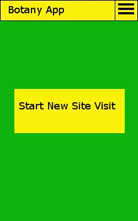
\includegraphics[scale=1]{uiDesign/botanyAppNewSiteVisit1.png}
            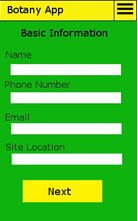
\includegraphics[scale=1]{uiDesign/botanyAppNewSiteVisit2.png}
            \caption{An example new site visit form}
            \label{fig:newSiteVisit}
        \end{figure}

        \begin{figure}
            \centering
            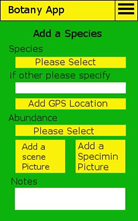
\includegraphics[scale=1]{uiDesign/botanyAppAddSpecies1.png}
            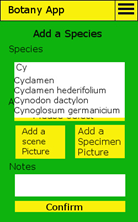
\includegraphics[scale=1]{uiDesign/botanyAppAddSpecies2.png}
            \caption{An example new species form}
            \label{fig:newSpecies}
        \end{figure}

        \begin{figure}
            \centering
            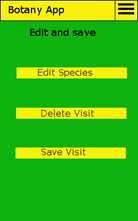
\includegraphics[scale=1]{uiDesign/botanyAppEditSaveSiteVisit.png}
            \caption{An example site/visit confirmation screen}
            \label{fig:editSaveSite}
        \end{figure}

        \begin{landscape}
            \begin{figure}
                \centering
                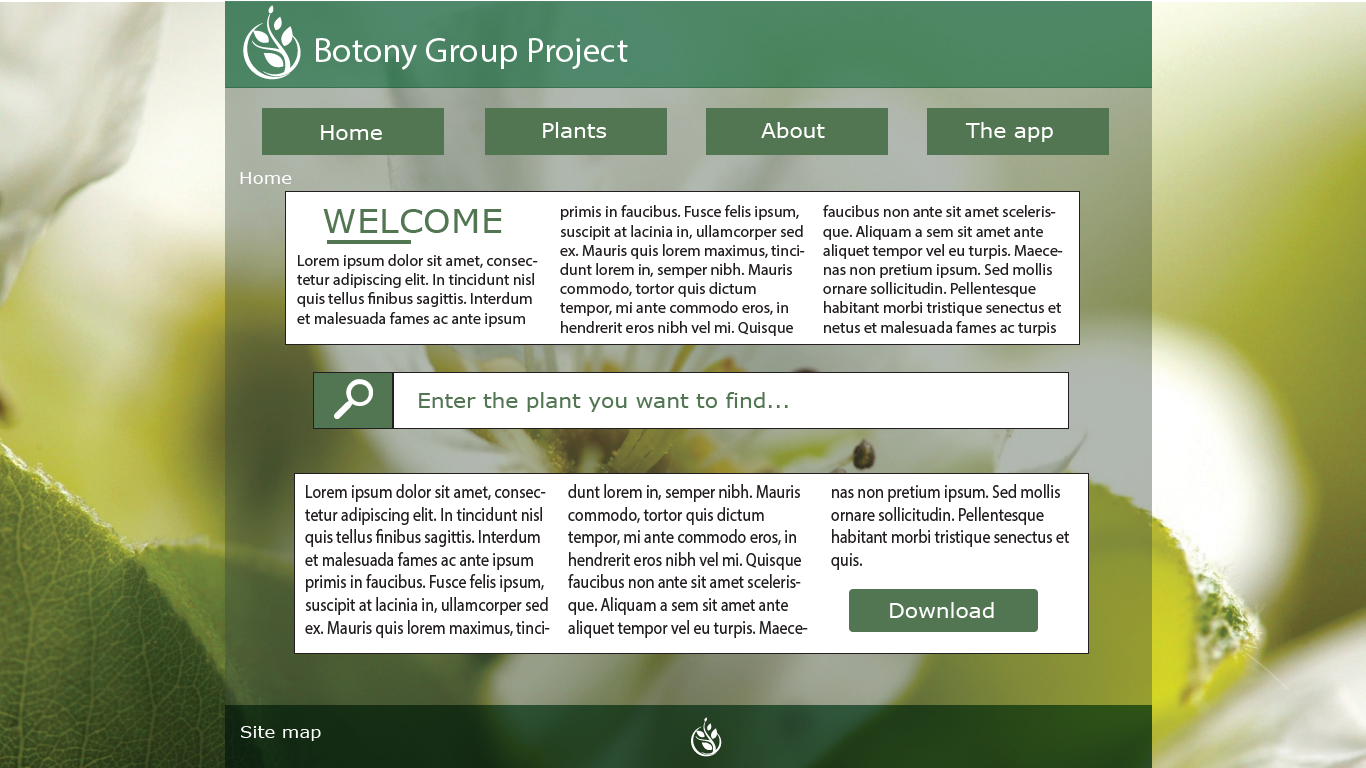
\includegraphics[scale=0.4]{uiDesign/uiwebimages/index.png}
                \caption{index.php}
                \label{fig:indexWebpage}
            \end{figure}

            \begin{figure}
                \centering
                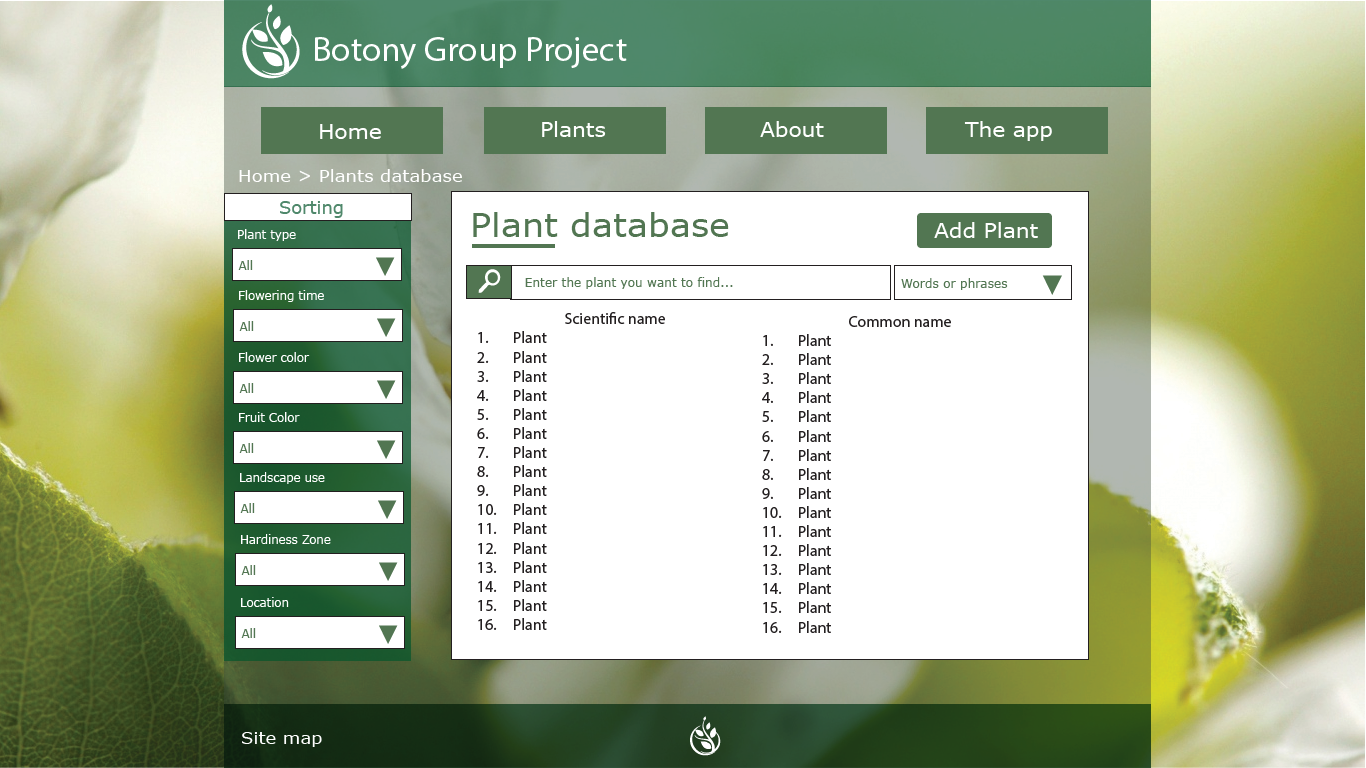
\includegraphics[scale=0.4]{uiDesign/uiwebimages/plantdb.png}
                \caption{An example of the plant database}
                \label{fig:plantDbWeb}
            \end{figure}

            \begin{figure}
                \centering
                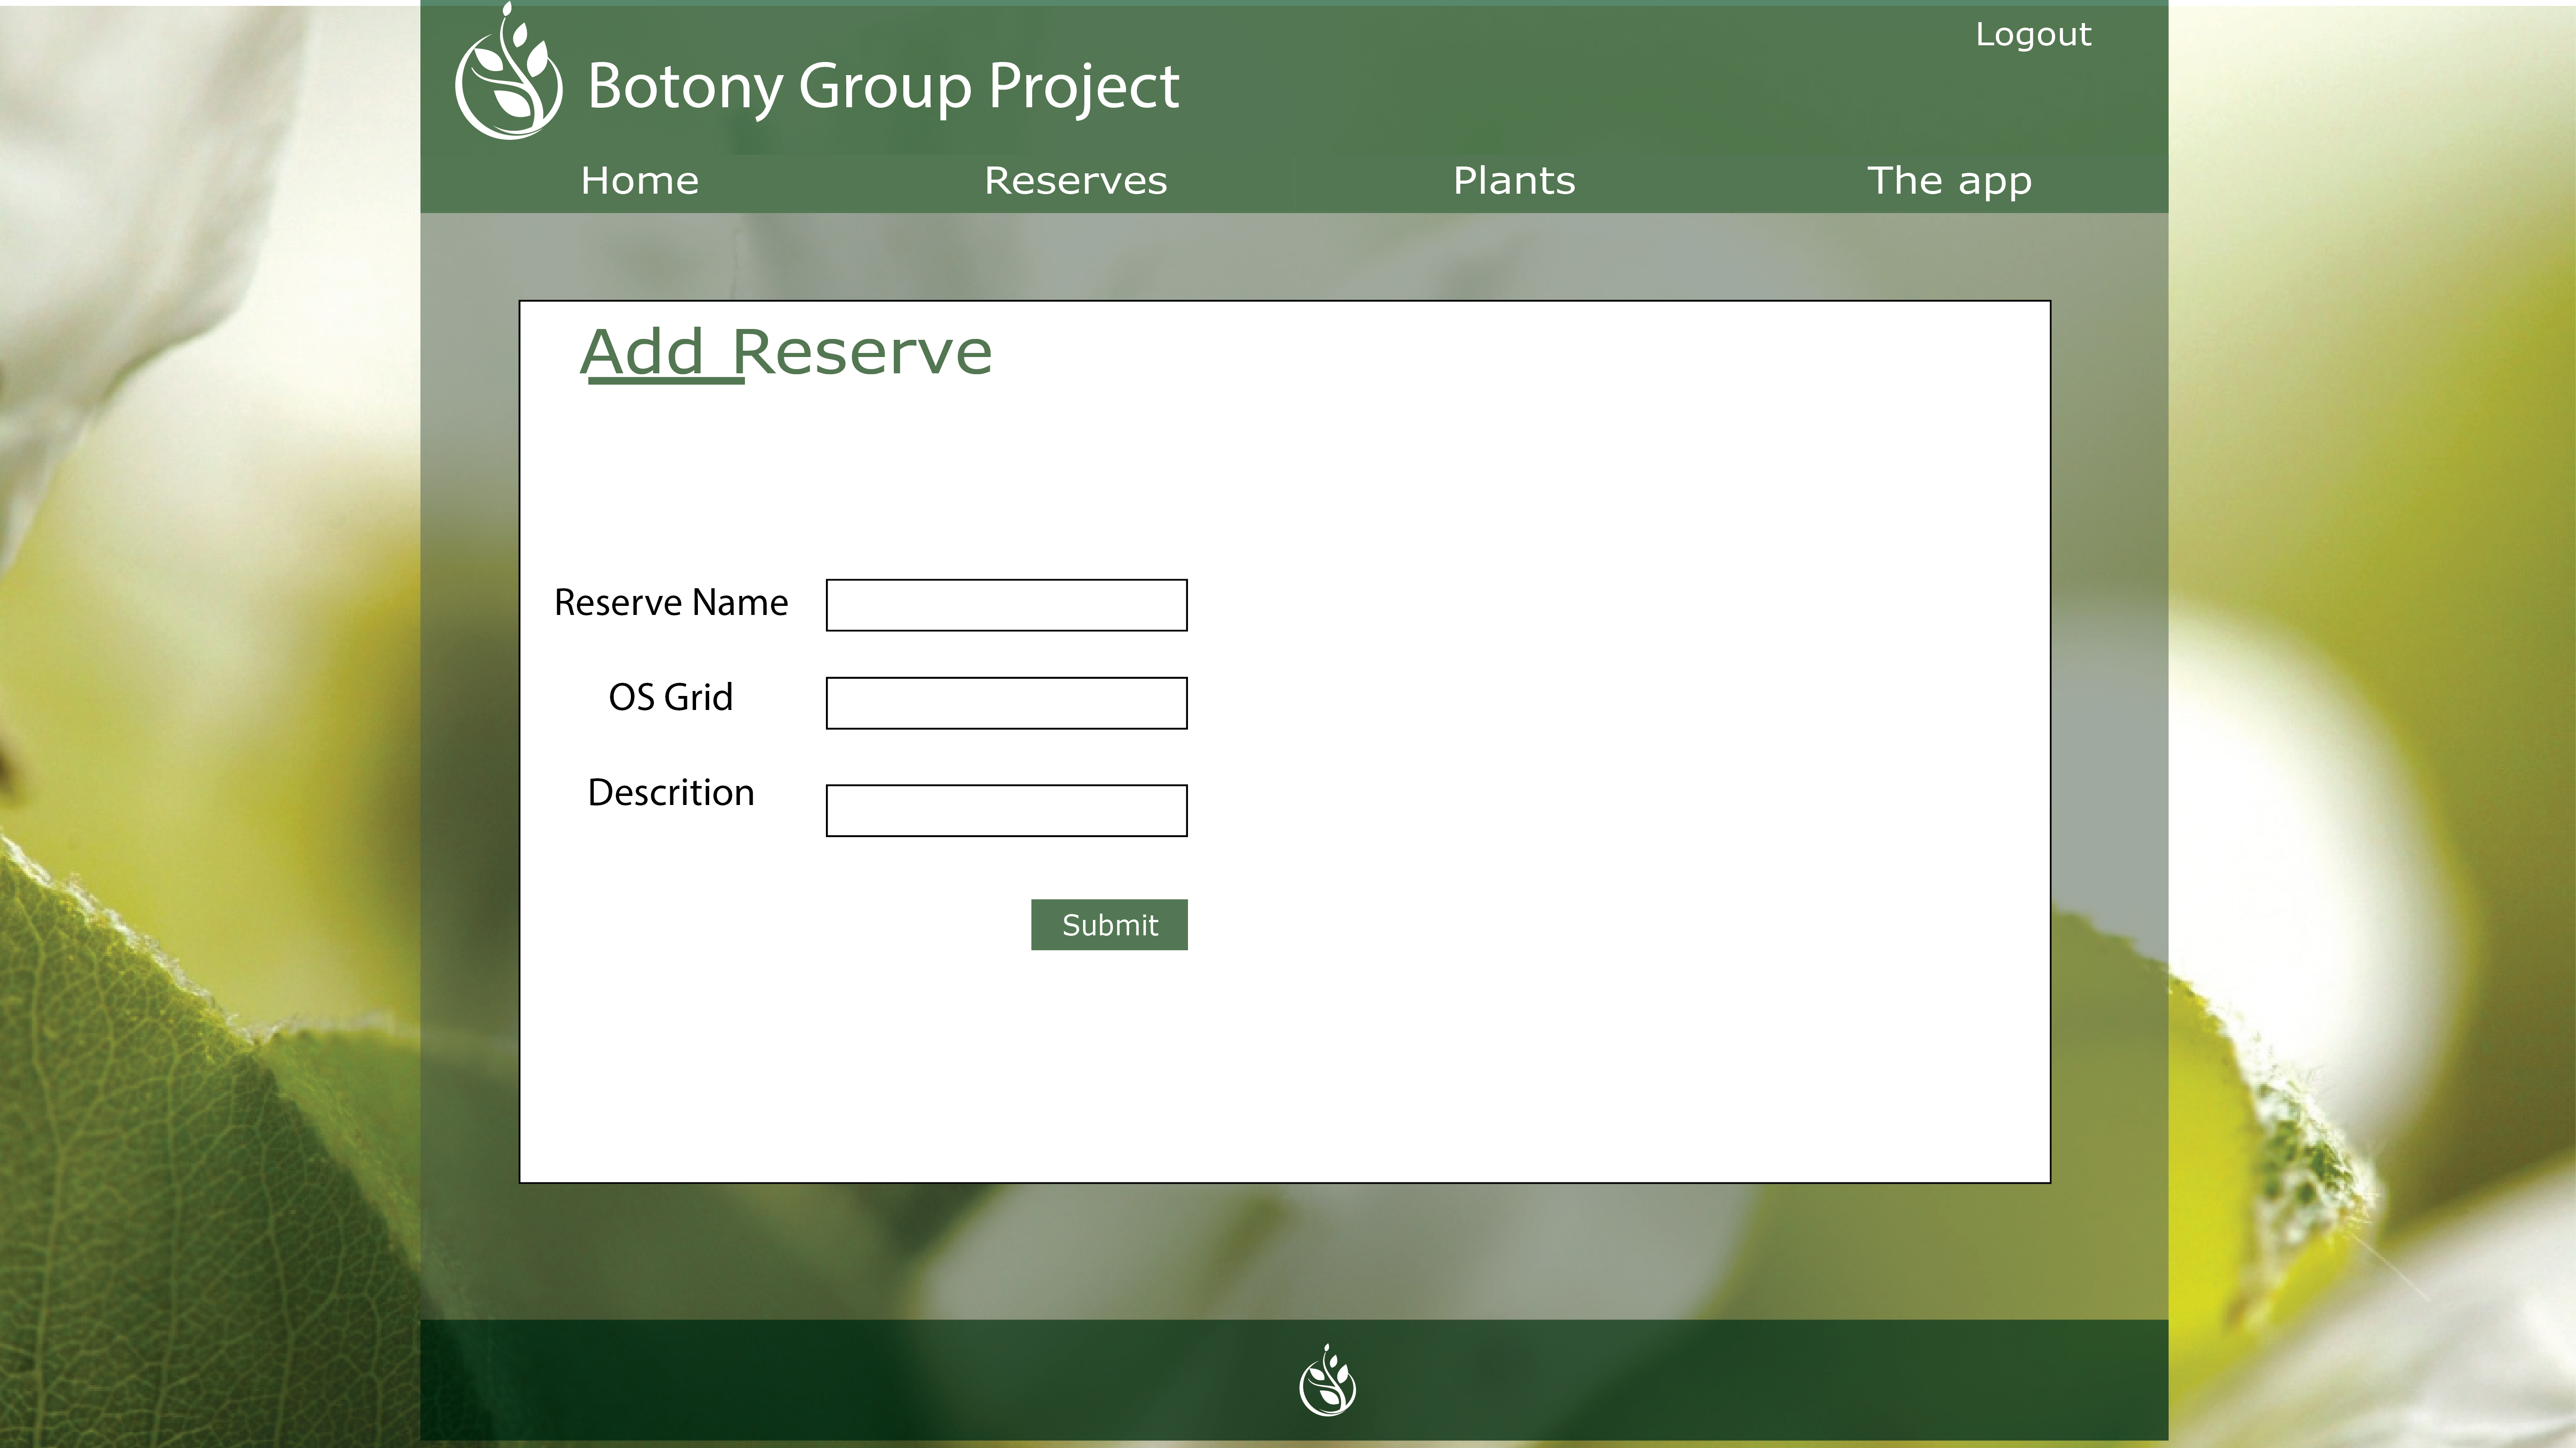
\includegraphics[scale=0.4]{uiwebimages/addreserve.png}
                \caption{An example plant entry in the site}
                \label{fig:viewWeb}
            \end{figure}

            \begin{figure}
                \centering
                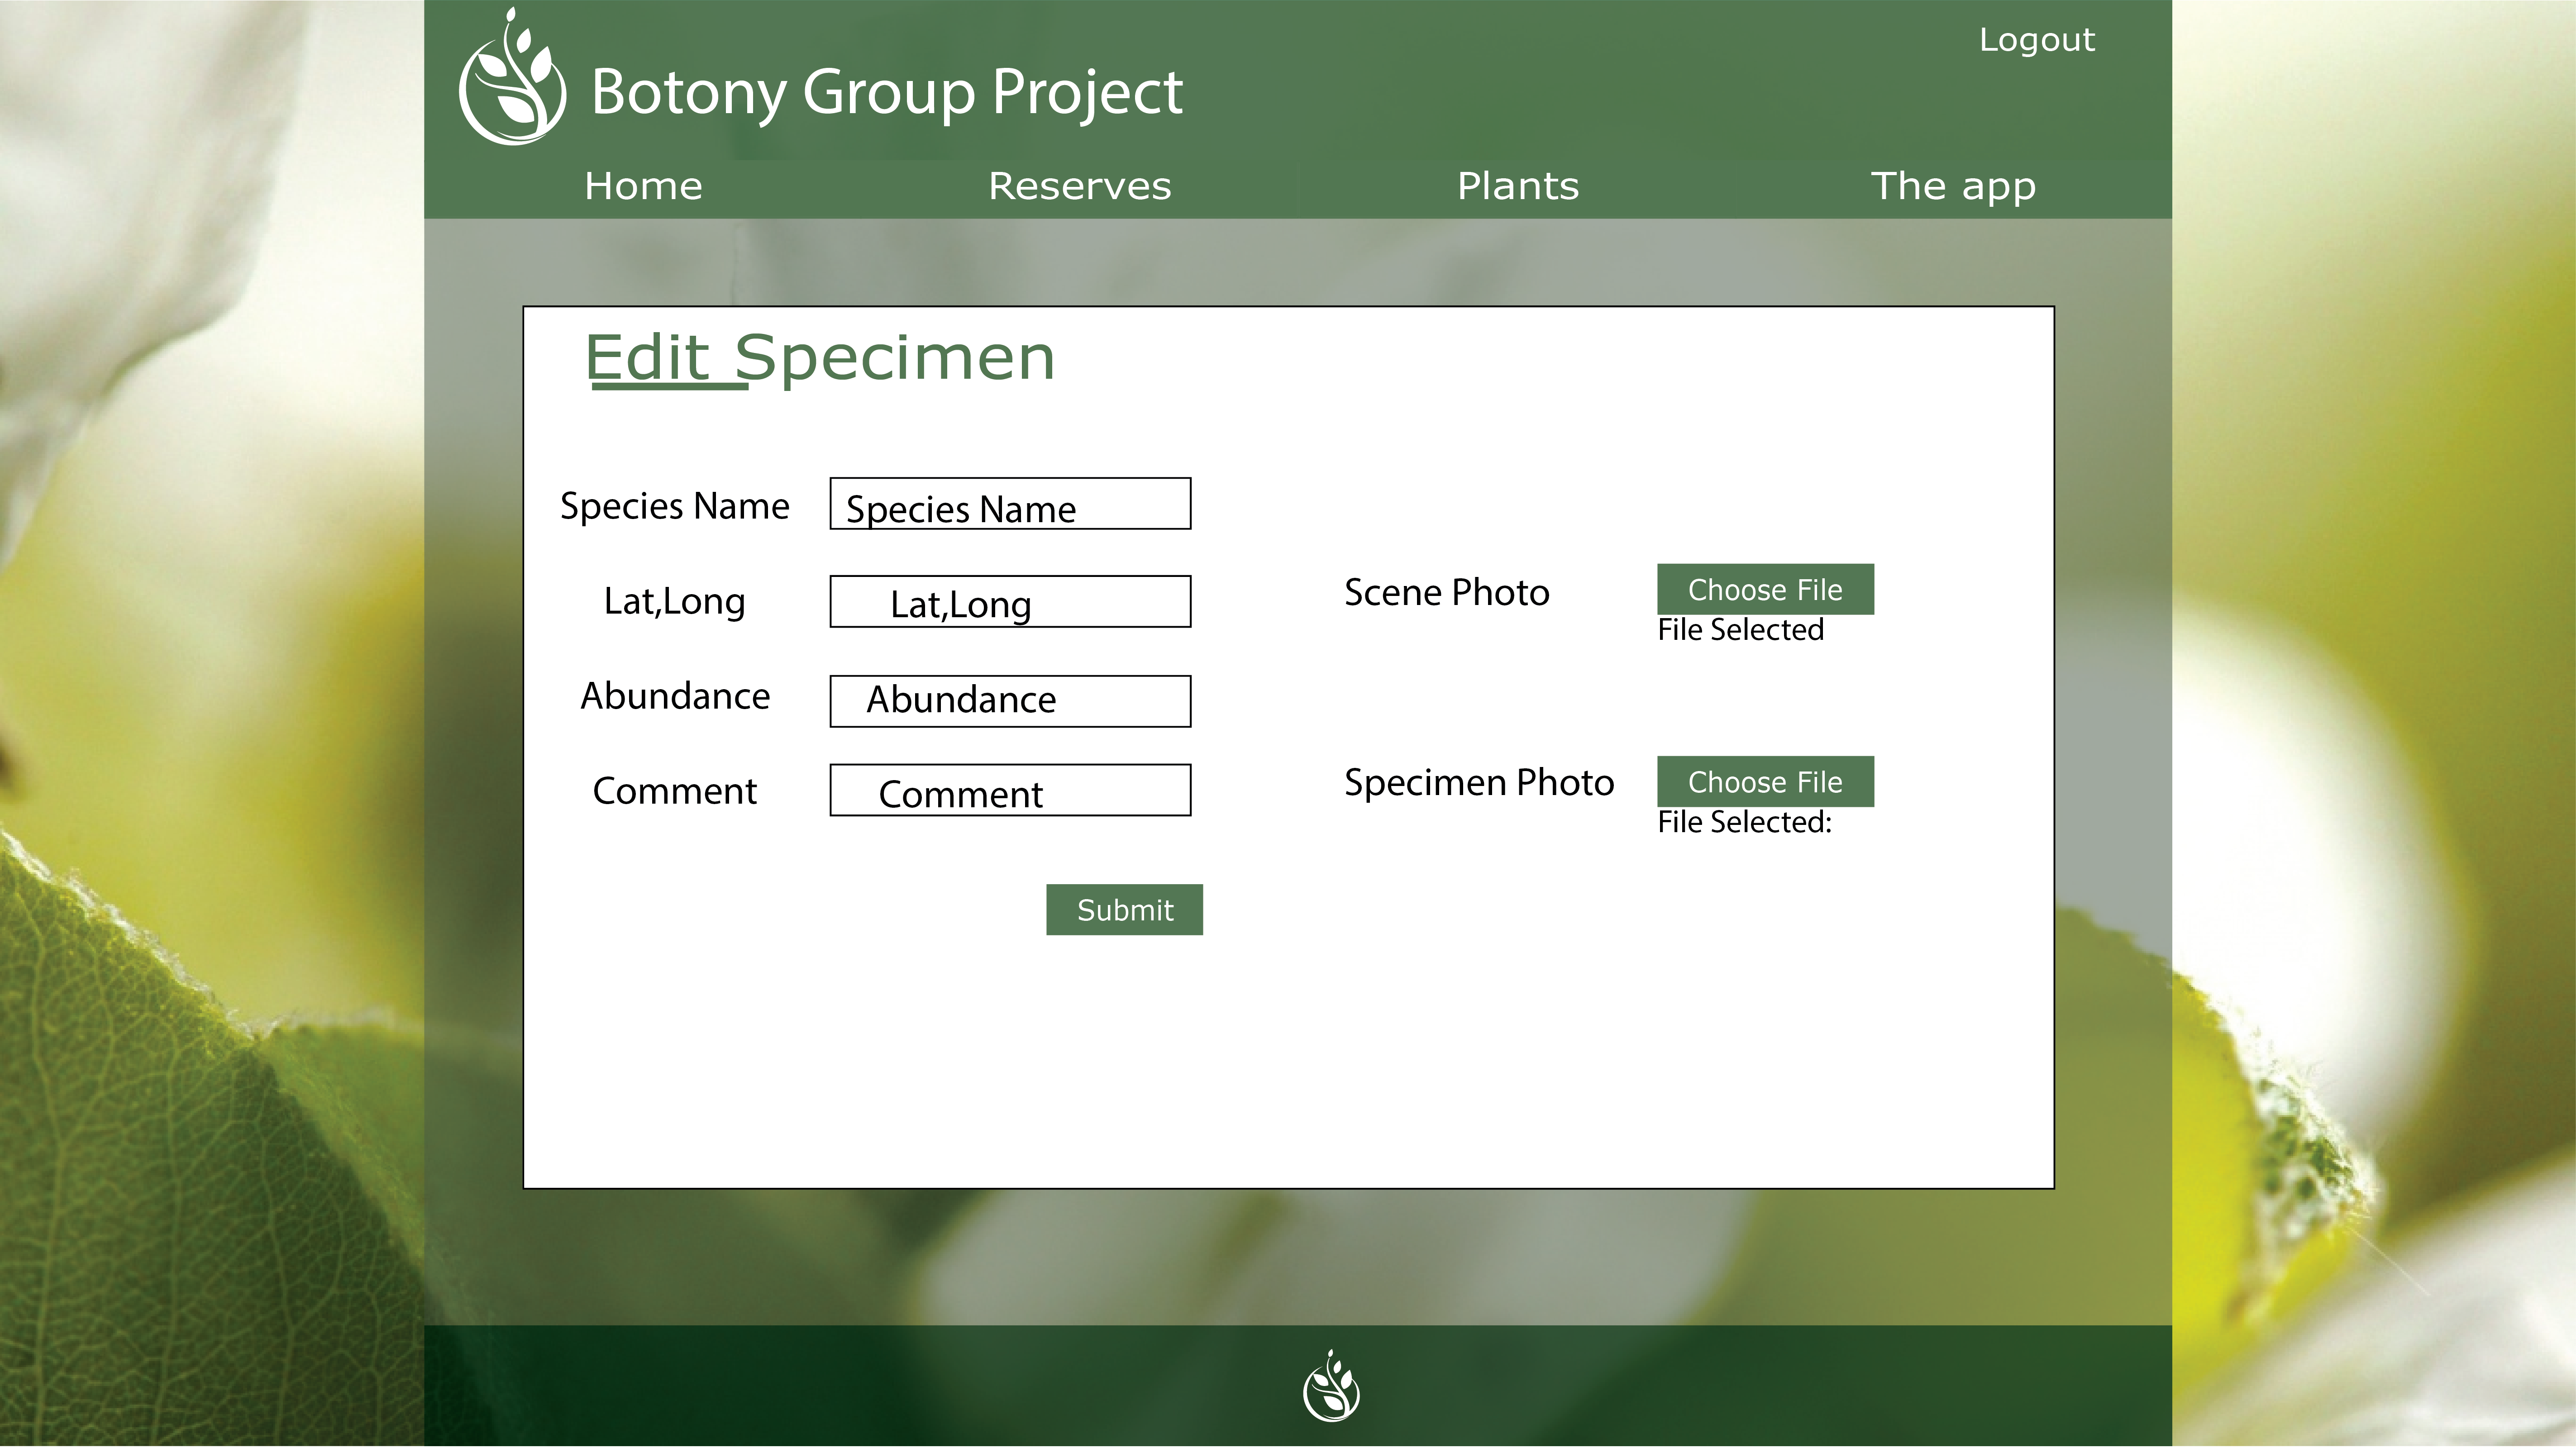
\includegraphics[scale=0.4]{uiwebimages/editspecimen.png}
                \caption{An example of a plant entry in edit mode}
                \label{fig:editWeb}
           \end{figure}

            \begin{figure}
                \centering
                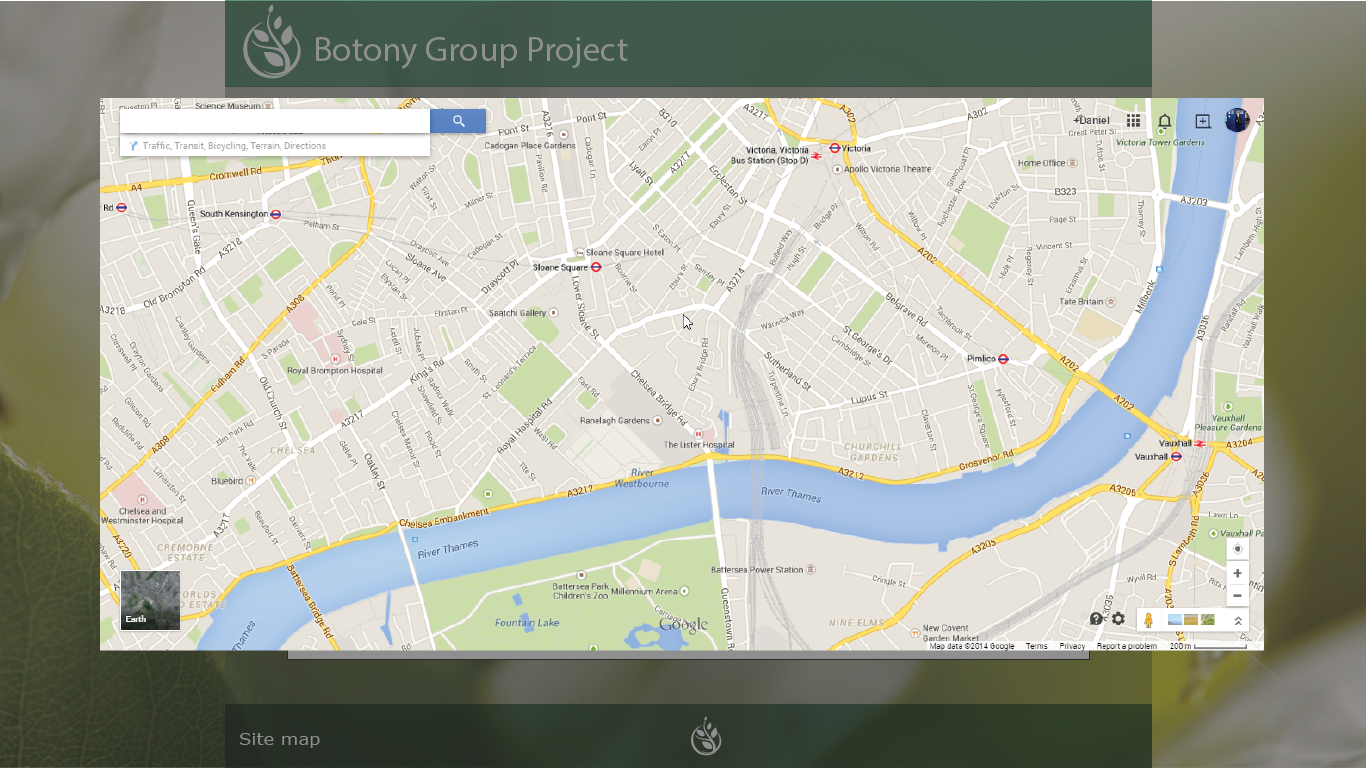
\includegraphics[scale=0.4]{uiDesign/uiwebimages/map.png}
                \caption{An example map to display recording locations}
                \label{fig:mapWeb}
            \end{figure}
        \end{landscape}